\begin{recipe}
    [% 
        preparationtime = {\unit[1]{h}},
        bakingtime = {\unit[50]{min}},
        portion = {\portion{4}},
        source = {jadlonomia.pl: krem-pomidorowy-z-pieczonymi-paprykami}
    ]
    {Tomato \& roasted pepper cream}

    \ingredients{%
        6-8 & red peppers \\
        \unit[2]{kg} & tomatoes \\
        2-4 claws & garlic \\
        \unit[1 \nicefrac{1}{2}]{glass} & vegetable bullion \\
        \unit[1]{tbs.} & olive oil \\
        \unit[1]{tbs.} & lemon juice \\
        & salt\&pepper \\
        & croutons \\
        & fresh basil
    }

    \preparation{%
        \step Preheat the oven to \unit[200]{\textcelcius}. Cut the peppers in half and remove inedible parts.
        Put on a baking tray (use paper or non-stick tray) with skin facing upwards.
        Put whole tomatoes and whole garlic claws (in husks) on another tray.
        Roast for \unit[30-40]{minutes} until edges of the peppers get burned.
        Take both trays out.

        \step Put the roasted peppers in a small pot and cover with a lid for a quarter.
        This will make peeling them much easier.
        Heat up some olive in a pan, put in the roasted potatoes and the garlic squeezed out of its husks.
        Simmer for \unit[10-20]{minutes}.

        \step Remove skin from the peppers, make sure to get rid of the burned parts.
        Add to the tomatoes with bullion and lemon juice and blend into a smooth paste.
        Season with salt and pepper, serve hot with croutons, basil and olive oil.

        \step If you (as I do) can't stand the ostentatious veganism of this recipe, go for grated cheddar or better yet, chopped into small cubes.
    }

\end{recipe}

\begin{figure}[h]
    \centering
    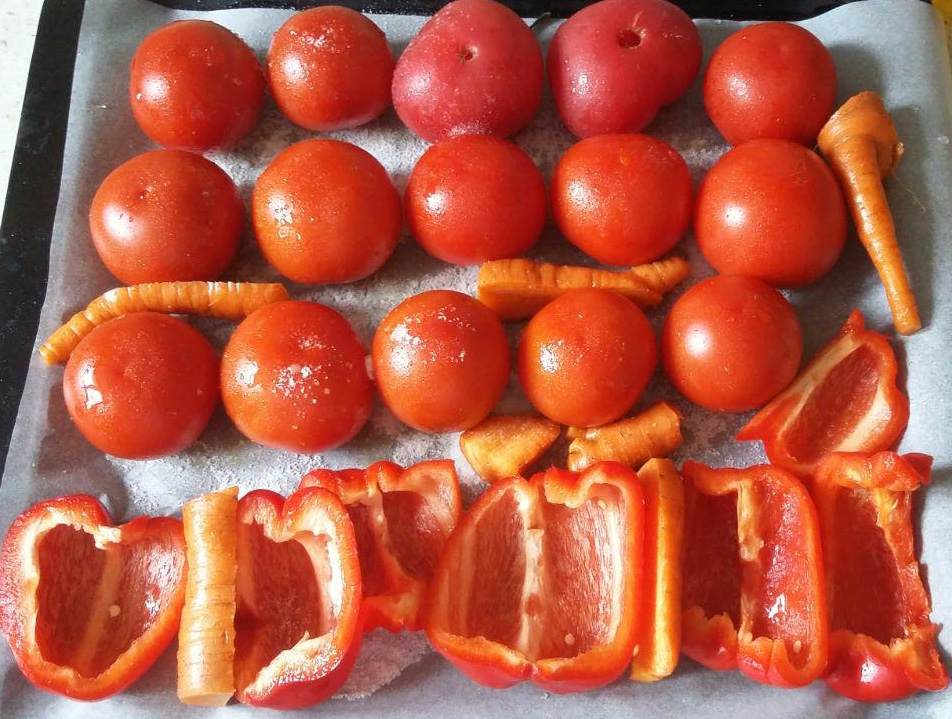
\includegraphics[width=6.5cm]{pic/roasted_peppers}
\end{figure}
